\section{Experimental Results}
\label{sec:eval}

\subsection{Experimental Setup}

%\subsubsection{Benchmark Generation}
In order to evaluate our extraction system automatically, we first design the benchmark
dataset. Test cases in benchmark are collected from the whole Internet. Our goal is to 
extract list items from the whole Internet and not to extract list items from 
particular websites.

In collection phrase, we use a paradigm-superlative Number Object- which indicates the web page contains a list of N items in the same topic. We first google an instance of the paradigm such as Best 10 Players, then we collect the search result using a heuristics. By using different instances of the paradigm, we collect 100 web pages from different websites and domains.

After collection, we label the cached web pages. 
For each web page, we label the first item of data record list which we want to extract.

Finally we generate two benchmarks $B1$ and $B2$
which have 92 pages and 96 pages respectively.
And there are no overlapping between them.

In order to compare with MDR\cite{LiuGZ03:MDR} system,
we generate another benchmark $B3$ 
from the testbed\cite{deepwebtestbed} 
which is used in Gengxin Miao's paper\cite{MiaoTHSM09:TagPathClustering}.
The testbed is designed for information extraction from the deep Web,
which has 253 Web pages from 51 web sites randomly with search forms.
We randomly choose 142 pages from 29 web sites to form $B3$.
Since our system needs to know the list item number $k$ of the page,
we manually assign the list number $k$ for each page in the benchmark.
Also we label the first item of data record list of each page.

%\subsubsection{Experimental Environment}
Our experiments were carried out on a Core (TM) 2 computer
with a 2GHz Duo CPU and 3GB of RAM. 

\subsection{Effect of Optimizations}

Given a page $p$ for evaluation, 
we have the extracted list items $S_l$. 
If one of the items in $S_l$ contains our manually added label, 
then we consider this page are extracted correctly.

Here we use precision and recall as the evaluation metrics for our system's accuracy test. 
The precision($P$) and recall($R$) are defined straightforwardly as follows:

\begin{equation}
	P = \frac{|{\rm correctly\,extracted\,pages}|}{|{\rm pages\,with\,returned\,list\,items}|}
\end{equation}

\begin{equation}
	R = \frac{|{\rm correctly\,extracted\,pages}|}{|{\rm number\,of\,testcases\,in\,benchmark}|}
\end{equation}

We compare the performance of two versions of our system.
the basic and the optimized.
The result of the experiment is shown in Figure \ref{fig:PR} and 
the average accuracy statistics are shown in Table \ref{tab:EvalRes1}.

\begin{table}[tb]
\centering
\caption{Average Accuracy Comparison}
\label{tab:EvalRes1}
\begin{tabular}{|c||c|c|} 
\hline
Version & $ P$(\%) & $R$(\%)\\\hline \hline
Basic & 87.3 & 59.5 \\\hline
Optimized & {\bf 90.3} & {\bf 70.9} \\\hline
\end{tabular}
\end{table}

\begin{figure}[th]
	\centering
	\epsfig{file=./pic/PR.eps,width=0.9\columnwidth}
	\caption{Precision and Recall for Each Benchmark}
	\label{fig:PR}
\end{figure}

The result indicates that the optimizations can remarkably improve the performance,
especially of the recall score. 
Thus, the accuracy our final system is satisfying 
and sufficient for solving our problem.

We also record the average running time for each step to test efficiency, 
which is listed in Table \ref{tab:TimeCostDistribution}.
The data shows the high efficiency of our system,
the algorithm and optimization only take up about one third of total running time.
Besides, the optimized system has a shorter running time than the basic one, 
which indicates those optimizations won't harm the efficiency of the whole system.
\begin{table}[tb]
\centering
\caption{Average Execution Time of Different Stages}
\label{tab:TimeCostDistribution}
\begin{tabular}{|c||c||c|c|c|c|} 
\hline
Version & Total & I/O & Parsing & Algorithm & Optimization \\\hline \hline
Basic(ms) & 402.9 & 141.5 & 115.8 & 145.6 & 0\\\hline
Optimized(ms) & 374.7 & 141.6 & 116.2 & {\bf116.4} & {\bf0.5}\\\hline
\end{tabular}
\end{table}

Also, we conduct a scaling test of file size,
which is shown in Figure \ref{fig:FileSize}.
The test set are 120 pages with proper size from $B1$ and $B2$.
The result shows a certain positive correlation between file size and running time.

\begin{figure}[th]
	\centering
	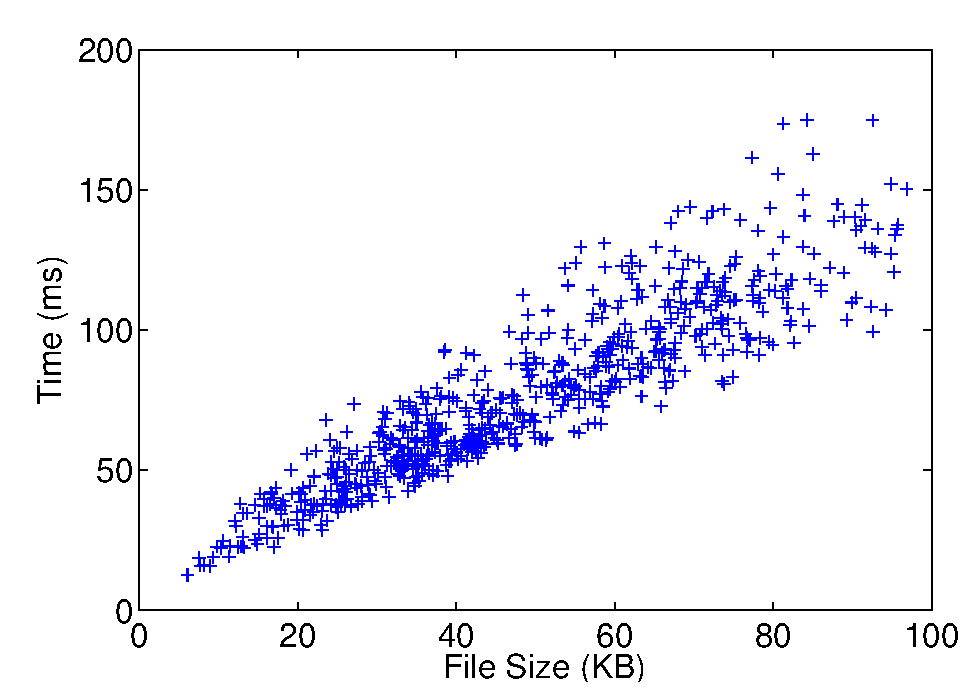
\epsfig{file=./pic/filesize.eps,width=0.9\columnwidth}
	\caption{Scaling Test of File Size}
	\label{fig:FileSize}
\end{figure}

%We also calculate the average time for the pages of the same list size, and plot them in
%\ref{fig:ListSize}, which show that list size doesn't affect execution time.

%\begin{figure}[th]
%	\centering
%	\epsfig{file=./pic/listsize.eps,width=0.9\columnwidth}
%	\caption{Scaling Test of List Size}
%	\label{fig:ListSize}
%\end{figure}

\subsection{Peer Comparison}

When comparing with MDR, we would like to introduce the evaluation metrics
used in Miao's work\cite{MiaoTHSM09:TagPathClustering}.
The meaning of precision and recall is a little different which is defined as
$P^*$ and $R^*$.
The {\rm ground\,truth} are all the list items of a Web site,
{\rm true\,positives} are the list items correctly extracted
and {\rm false\,positives} are the list items that incorrectly included in the same list with {\rm true\,positives}.
For the case that both false and true positives equal to 0, we define $P^*$ to be zero.

\begin{equation}
	P^* = \frac{|{\rm true\,positives}|}{|{\rm true\,positives}|+|{\rm false\,positives}|}
\end{equation}

\begin{equation} 
	R^* = \frac{|{\rm true\,possitive}|}{|{\rm ground\,truth}|}
\end{equation}

The result of the comparison is listed in Table \ref{tab:EvalRes2},
which shows that our system has an obviously higher precision and recall than
MDR system in B3. 
Furthermore, efficiency of the Optimized System is better since the average time is much shorter than MDR.
The experimental result of MDR is very close to that in Miao's work\cite{MiaoTHSM09:TagPathClustering}
($P^*=59.8\%$ and $R^*=61.8\%$), which infers the validity of the experiment.

\begin{table}[tb]
\centering
\caption{Peer Comparison}
\label{tab:EvalRes2}
\begin{tabular}{|c||c|c|c|} 
\hline
Version & $P^*$ (\%) & $R^*$ (\%) & Avg Time\\\hline \hline
Optimized & {\bf90.4} & {\bf73.2} & 144.4 ms \\\hline
MDR & 54.4 & 56.4 & 1-2 s \\\hline
\end{tabular}
\end{table}

We also tries to test MDR with $B1$ and $B2$. 
However, for more than half of the pages we test,
it takes more than 1 minute to give result.
Even if we omit those pages, 
the precision $P$ and recall $R$ are still very low($<15\%$),
which can not form any sensible comparison.
As a result, MDR system is not suitable for solving our problem.
